% Chapter 1

\chapter{Introducción General} % Main chapter title

\label{Chapter1} % For referencing the chapter elsewhere, use \ref{Chapter1} 
\label{IntroGeneral}

%----------------------------------------------------------------------------------------

% Define some commands to keep the formatting separated from the content 
\newcommand{\keyword}[1]{\textbf{#1}}
\newcommand{\tabhead}[1]{\textbf{#1}}
\newcommand{\code}[1]{\texttt{#1}}
\newcommand{\file}[1]{\texttt{\bfseries#1}}
\newcommand{\option}[1]{\texttt{\itshape#1}}
\newcommand{\grados}{$^{\circ}$}

%----------------------------------------------------------------------------------------

%\section{Introducción}

%----------------------------------------------------------------------------------------
\section{Proceso de Galvanización en PCBs}

En el proceso de galvanización de pistas y vías de un PCBs el control de los parámetros físicos en cada una de las etapas es fundamental para garantizar la uniformidad del cobre. Este proceso consiste en la inmersión de los placas en distintos baños químicos que se observan en la Figura \ref{fig:thr_correcto}, y en la Figura \ref{fig:thr_correcto_perfil} el resultado de un correcto proceso donde el espesor del cobre conductor es uniforme en toda la cavidad.

\begin{figure}[h]
	\centering
	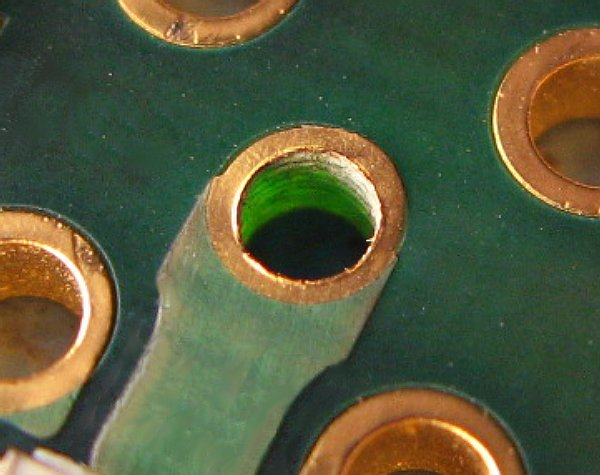
\includegraphics[width=.5\textwidth]{Figures/through_hole_correcto}
	\caption{Via con galvanización correcto en un PCB}
	\label{fig:thr_correcto}
\end{figure}

\begin{figure}[h]
\centering
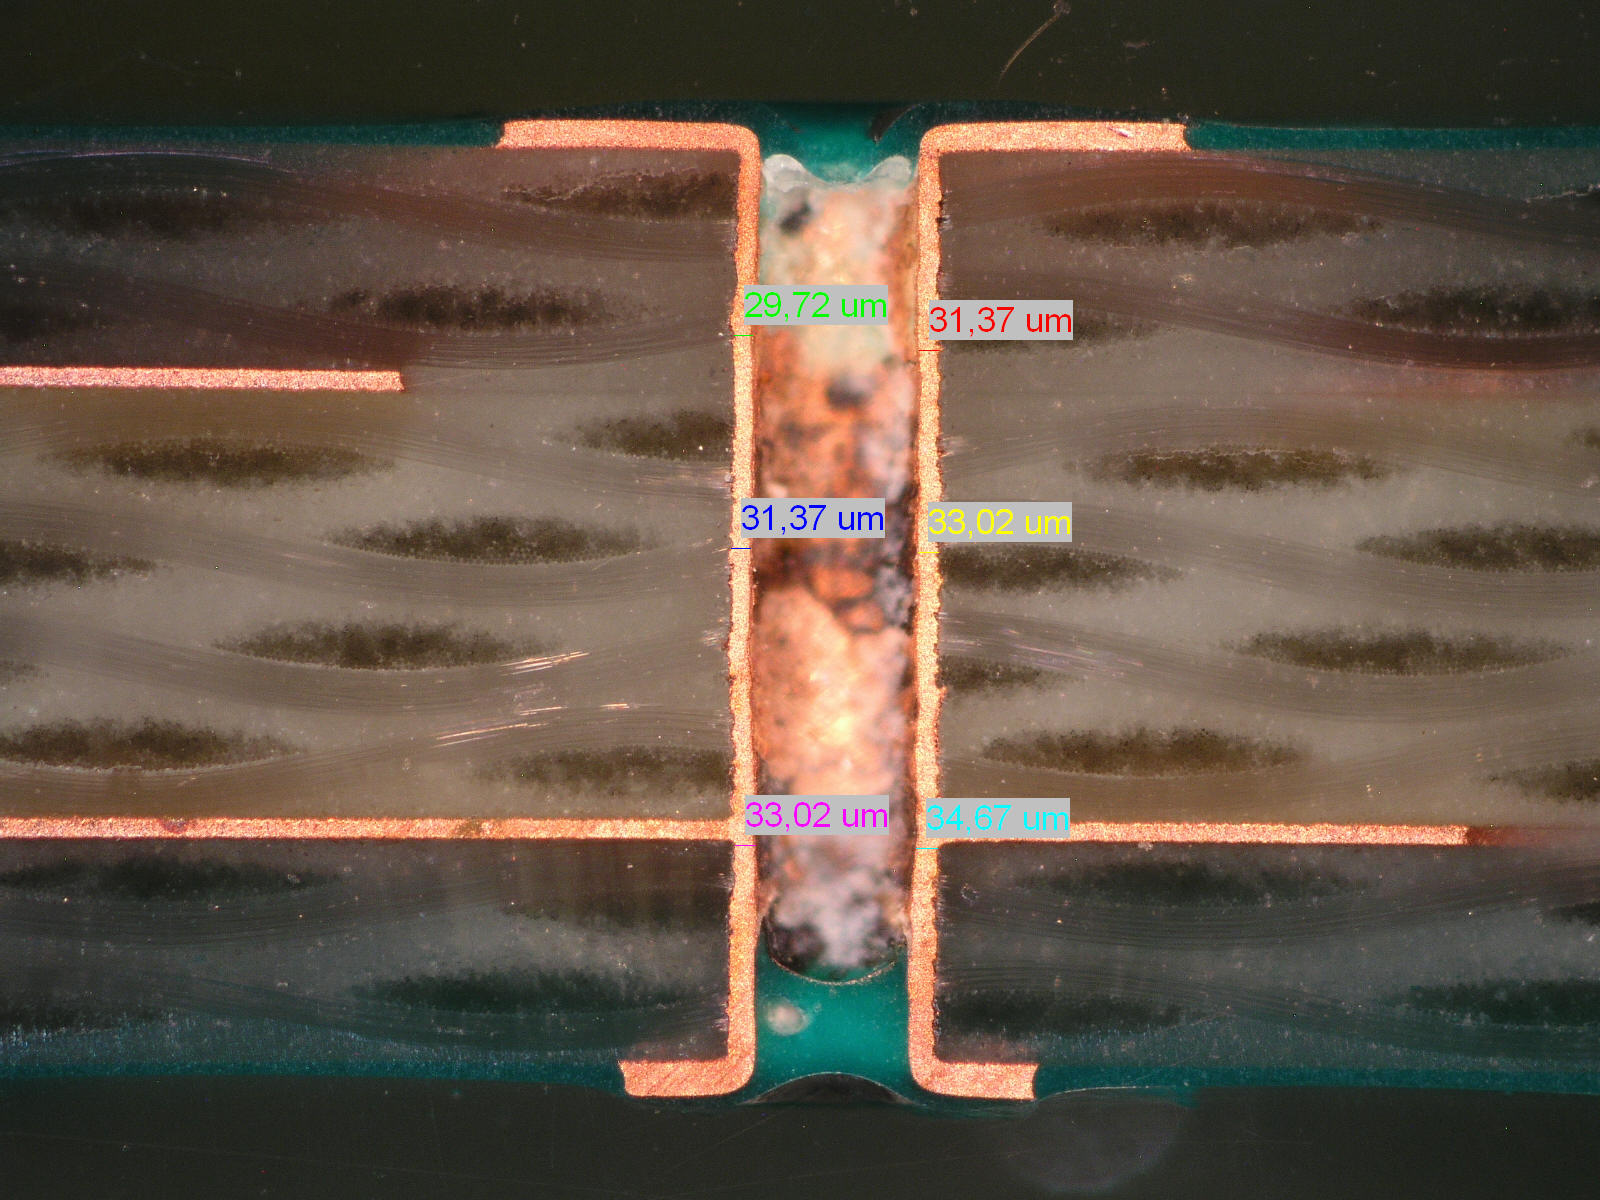
\includegraphics[width=.5\textwidth]{Figures/through_hole_perfil}
\caption{Perfil de una via correctamente galvanizada}
	\label{fig:thr_correcto_perfil}
\end{figure}

Cuando este proceso no ocurre correctamente se originan distintas fallas, donde las más comunes son: vías sin galvanizar, vías obstruidas por exceso de cobre y capa no uniforme de metal cobre en la vía con riesgo de no conductividad. En la Figura \ref{thr_incorrecto_perfil} se observan las distintos grosores de cobre en vias mal galvanizadas en función de su ubicación en el sustrato del PCB.

\begin{figure}[h]
	\centering
	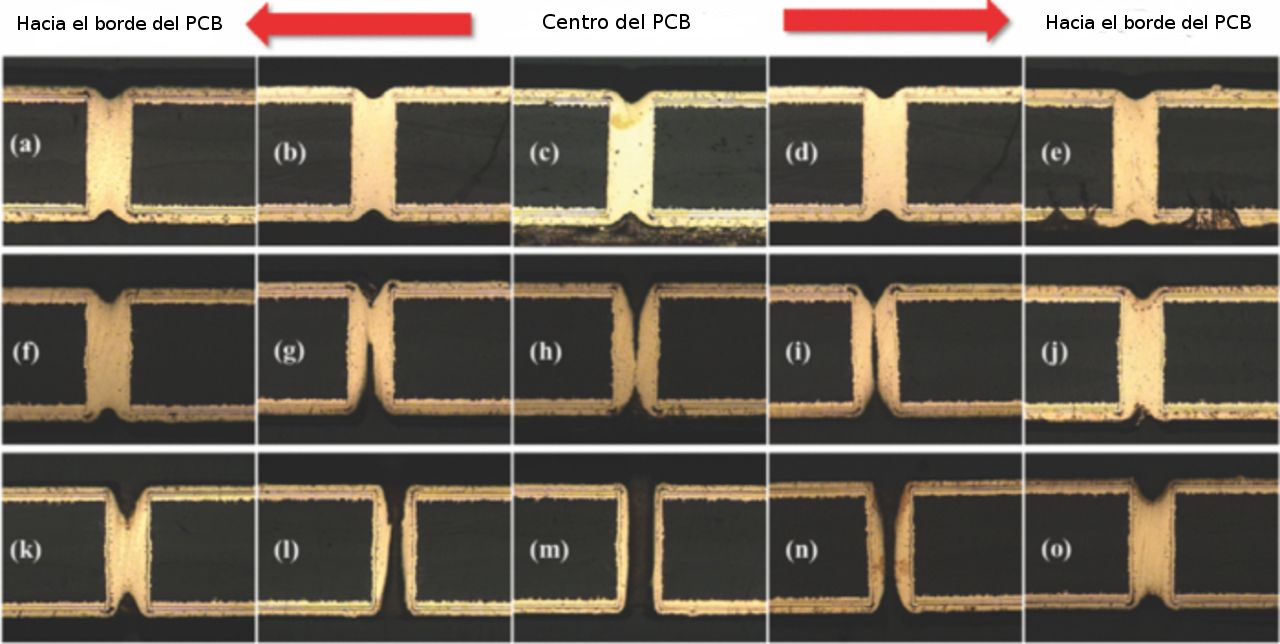
\includegraphics[width=.8\textwidth]{Figures/through_hole_perfil_fallado}
	\caption{Perfil un conjunto de sustratos con vías mal galvanizadas}
	\label{fig:thr_incorrecto_perfil}
\end{figure}

El proceso requiere una sucesión de baños por distintas soluciones químicas y enjuagues en agua, previas y después del proceso de electrolisis con cobre sobre el sustrato. En la Figura \ref{fig:diagrama_proceso} se resumen los pasos de forma simplificada, en el proceso de PCB se utilizan mas de 10 etapas.

\begin{figure}[h]
	\centering
	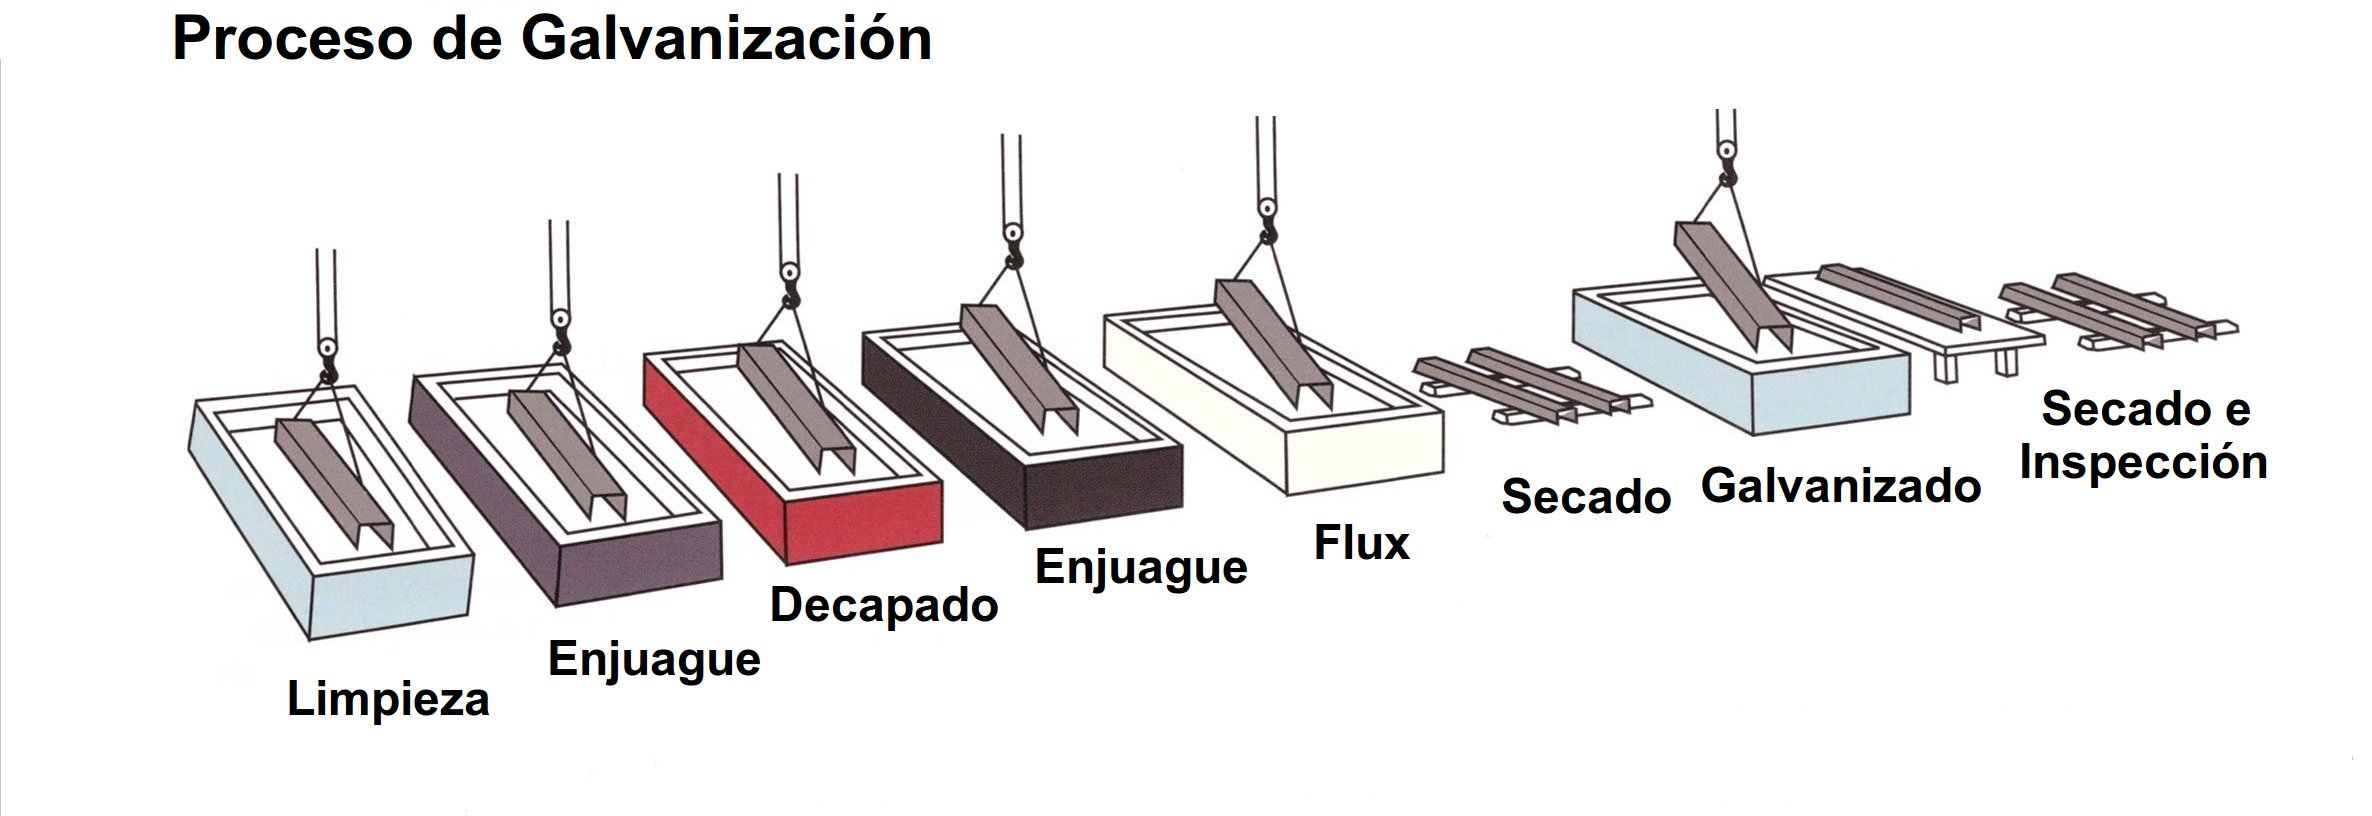
\includegraphics[width=.8\textwidth]{Figures/diagrama_galvanizado_castellano}
	\caption{Diagrama simplificado de una linea de galvanizado}
	\label{fig:diagrama_proceso}
\end{figure}


\LaTeX{} no es \textsc{WYSIWYG} (What You See is What You Get), a diferencia de los procesadores de texto como Microsoft Word o Pages de Apple o incluso LibreOffice en el mundo open-source. En lugar de ello, un documento escrito para \LaTeX{} es en realidad un archivo de texto simple, llano que \emph{no contiene formato} . Nosotros le decimos a \LaTeX{} cómo deseamos que se aplique el formato en el documento final escribiendo comandos simples entre el texto, por ejemplo, si quiero usar \emph{texto en cursiva para dar énfasis}, escribo \verb|\emph{texto}| y pongo el texto en cursiva que quiero entre medio de las llaves. Esto significa que \LaTeX{} es un lenguaje del tipo \enquote{mark-up}, muy parecido a HTML.

\section{Motivación y objetivo}

A partir de la búsqueda de incrementar los niveles de calidad en producto final surgió la necesidad de agregar control y monitoreo a determinadas bateas criticas en el proceso de modo de asistir a los operarios de planta en tiempo real sobre alguna anomalía en los parámetros antes de continuar con el proceso. En la Figura \ref{fig:planta_actual} se puede ver como es la linea de proceso actual.

\begin{figure}[h]
	\centering
	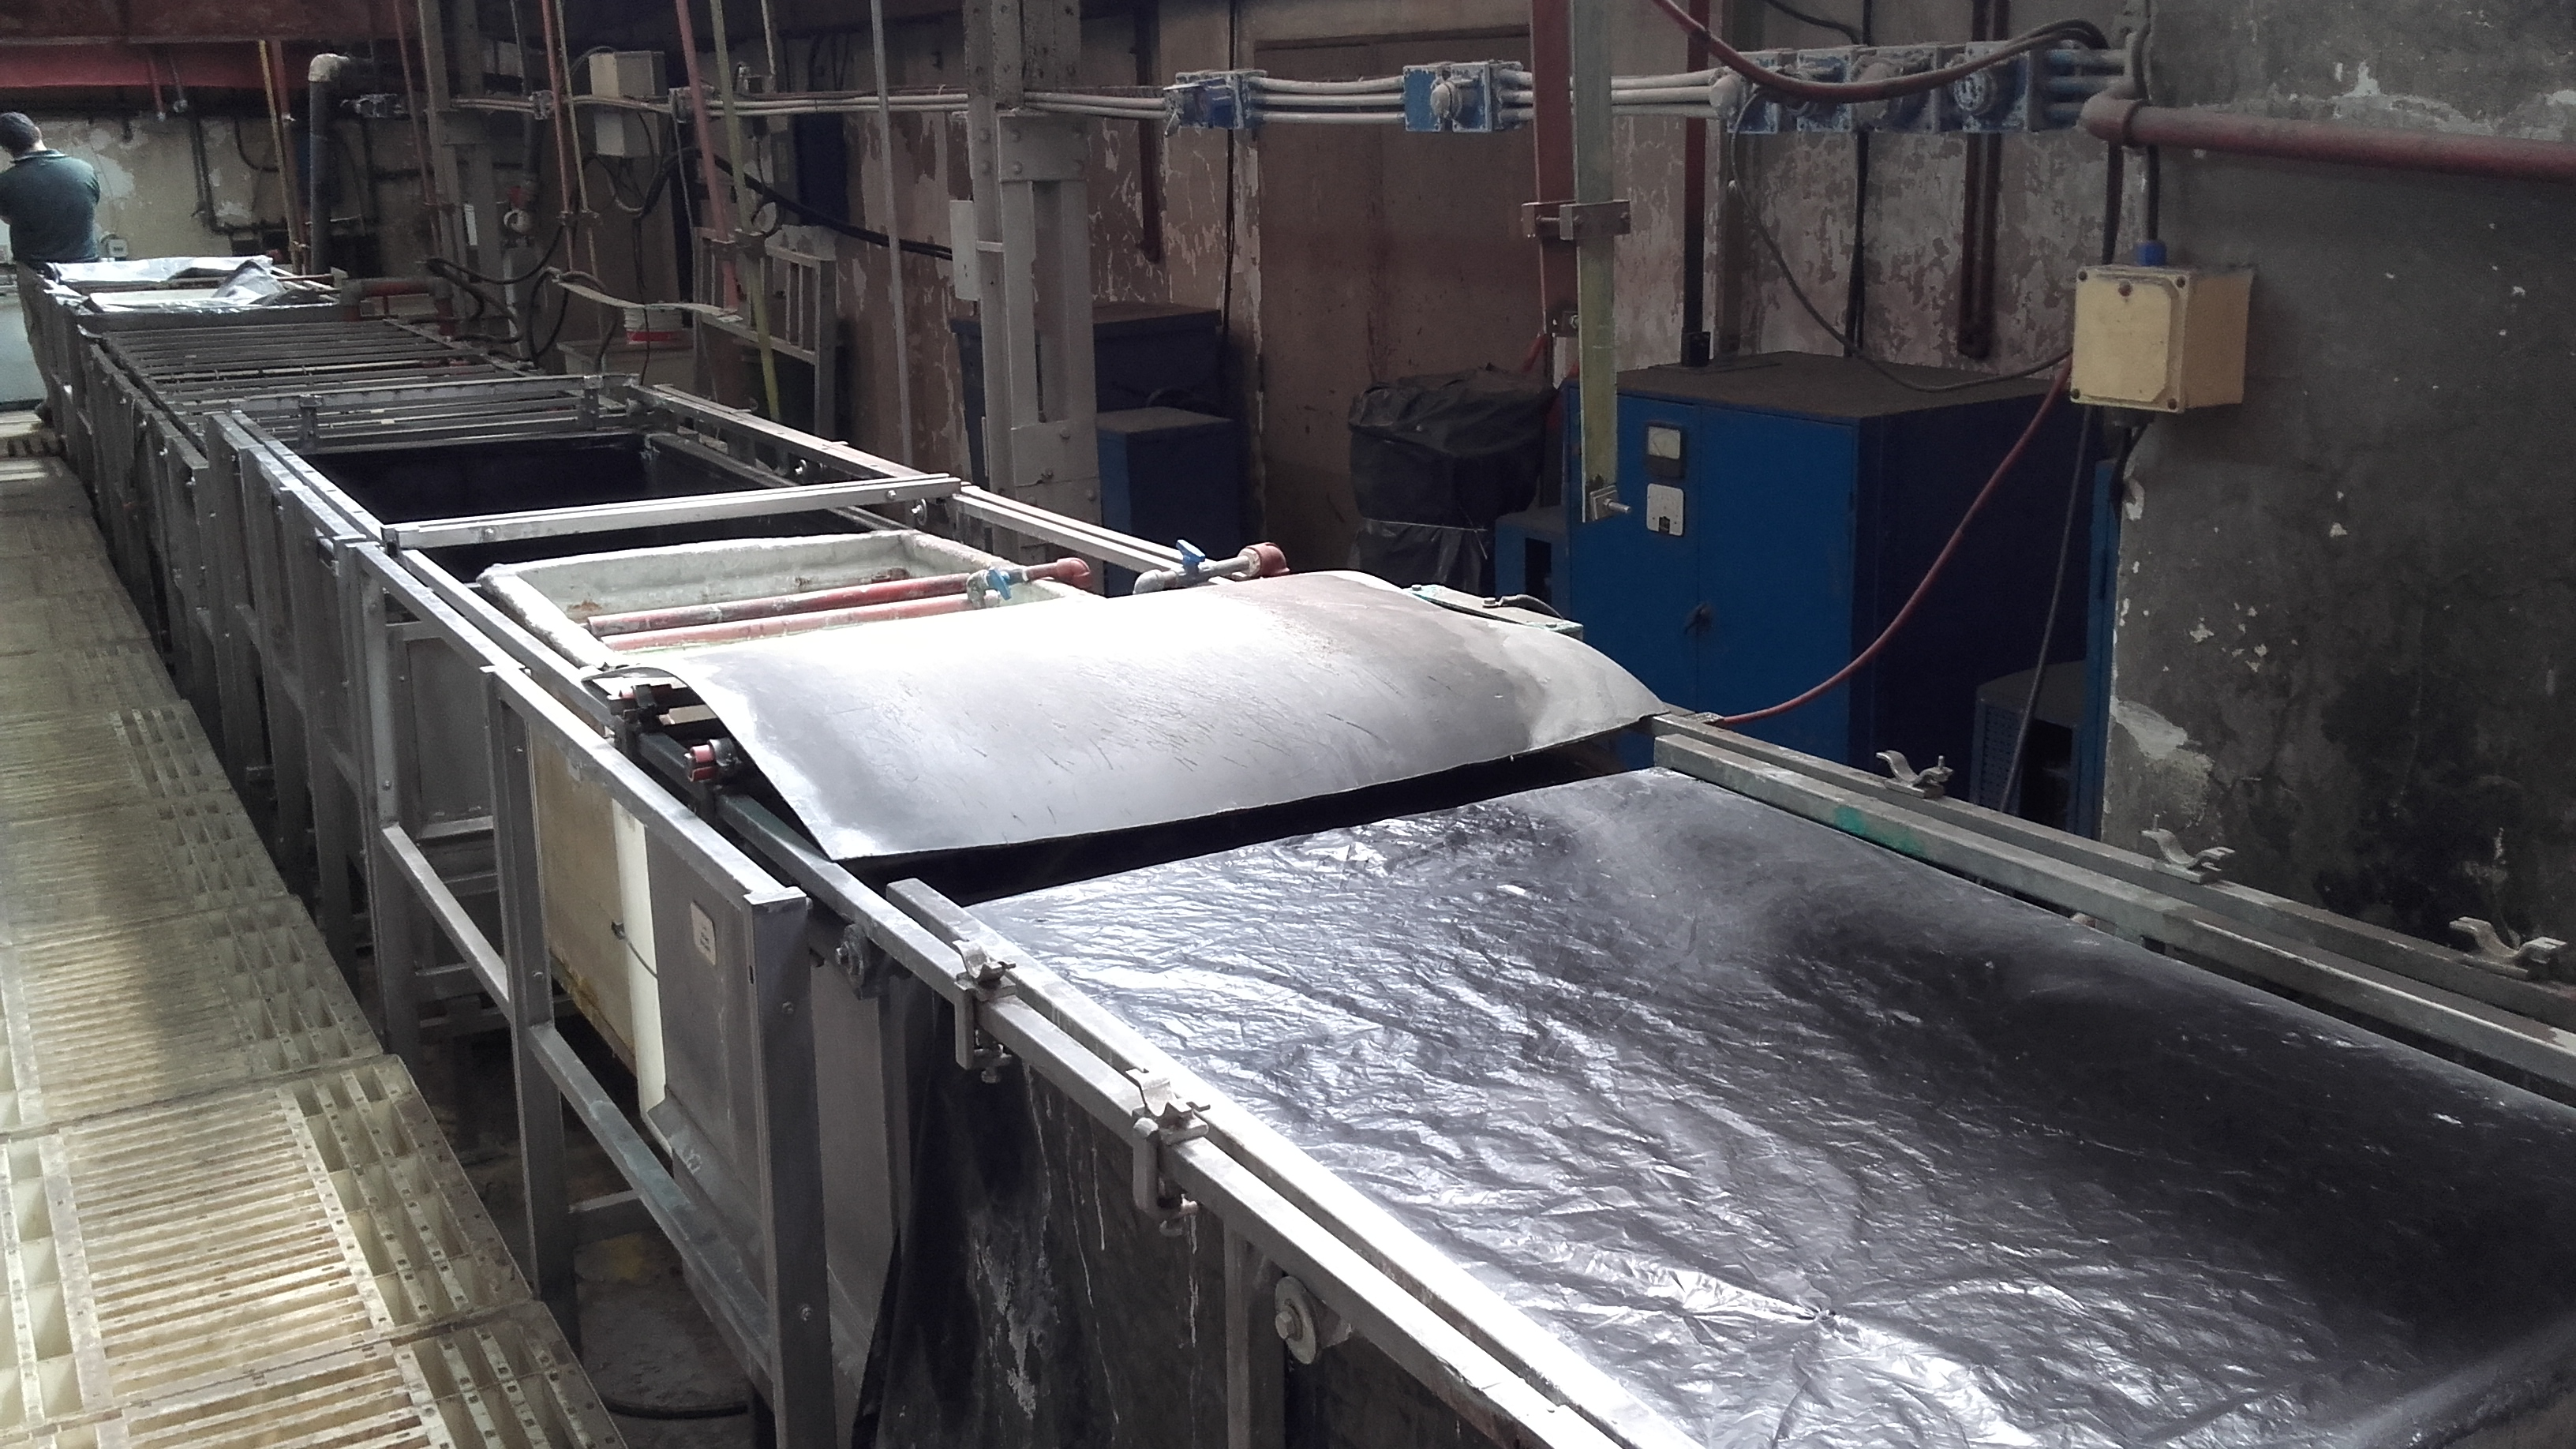
\includegraphics[width=.8\textwidth]{Figures/planta_actual}
	\caption{Linea de galvanizada actual operada manualmente}
	\label{fig:planta_actual}
\end{figure}

Como segundo objetivo como el proceso actual es totalmente hecho a mano y se esta trabajando en modernizarla y cambiarla de lugar se busca que el mismo sistema pueda integrar a una linea de traslación de los PCBs automatizada, lo cual se logró con el conteo de tiempo de posicionamiento por etapa.  

Finalmente a modo de control general y auditoría se necesitaba que el sistema registre los valores de las parámetros de medición en archivos . 

Si usted es nuevo a \LaTeX{}, hay un muy buen libro electrónico - disponible gratuitamente en Internet como un archivo PDF - llamado, \enquote{A (not so short) Introduction to \LaTeX{}}. El título del libro es generalmente acortado a simplemente \emph{lshort}. Puede descargar la versión más reciente en inglés (ya que se actualiza de vez en cuando) desde aquí:
\url{http://www.ctan.org/tex-archive/info/lshort/english/lshort.pdf}

Está disponible en varios idiomas además del inglés. Se puede encontrar la versión en español en la lista en esta página: \url{http://www.ctan.org/tex-archive/info/lshort/}


\section{Objetivo}

El presente sistema embebido se focalizó en la confiabilidad, robustez y adaptabilidad con las interfaces eléctricas necesarias para que funcione en un ambiente industrial con los actuadores y sensores determinados por el cliente. Para tal fin se propuso que el mismo funcione sobre la plataforma eduCIAA en conjunto con una placa de interfaz hecha a medida, como un prototipo de prueba previo al desarrollo de un hardware propio.

\subsection{Alcance}

El proyecto incluyó los siguientes puntos:
\begin{itemize}
	\item Estudio preliminar de las arquitecturas adecuadas para la implementación del sistema principal y subsistemas.
	\item Diseño de alto nivel (arquitectura) del sistema.
	\item Diseño del sistema en lenguaje C para plataforma CIAA.
	\item Plan de pruebas unitarias y ensayos (testbenchs) para cada subsistema.
	\item Plan de pruebas de integración y ensayos (testbenchs) para agrupaciones de subsistemas.
	\item Plan de pruebas del sistema y ensayos (testbenchs) para el sistema completo.
	\item Documentación del sistema y subsistemas que incluye:
	\begin{enumerate}
		\item Descripción de entradas y salidas (frecuencias, tamaño y tipos de datos, señales de control, etc.)
		\item Descripción de parámetros del sistema.
		\item Requerimientos funcionales implementados trazables a los requerimientos del proyecto (matriz de trazabilidad).
		\item Hipótesis de diseño, justificación de la elección del diseño, estudios previos y marco teórico.
		\item Diagrama de arquitectura.
		\item Reporte de ensayos realizados.
		\item Referencias bibliográficas.
	\end{enumerate}
	\item Análisis y construcción del banco de pruebas.
\end{itemize}

El proyecto no incluyó: 
\begin{itemize}
	\item Estudio de los sensores y actuadores, se basará dicha información en los datos dados por el cliente. 
	\item Análisis de mejor solución para implementación de sistema de reporte remoto de variables y registros históricos. 
	\item Test del sistema en lugar de producción. La planta se encontraba en reestructuración y modernización.
\end{itemize}



%----------------------------------------------------------------------------------------

\section{Utilizando esta plantilla}

Si usted está familiarizado con \LaTeX{}, entonces puede explorar la estructura de directorios de esta plantilla y proceder a personalizarla agregando su información en el bloque \emph{INFORMACIÓN DE LA PORTADA} en el archivo \file{memoria.tex}.  

Se puede continuar luego modificando el resto de los archivos siguiendo los lineamientos que se describen en la sección \ref{sec:FillingFile} en la página \pageref{sec:FillingFile}.

Asegúrese de leer el capítulo \ref{Chapter2} acerca de las convenciones utilizadas para las Memoria de los Trabajos Finales de la Carrera de Especialización en Sistemas Embebidos de FIUBA.

Si es nuevo en \LaTeX{} se recomienda que continue leyendo el documento ya que contiene información básica para aprovechar el potencial de esta herramienta.

Si usted está escribiendo un documento con mucho contenido matemático, entonces es posible que desee leer el documento de la AMS (American Mathematical Society) llamado, \enquote{A Short Math Guide for \LaTeX{}}. Se puede encontrar en línea en el siguiente link: \url{http://www.ams.org/tex/amslatex.html} en la sección \enquote{Additional Documentation} hacia la parte inferior de la página.



\subsection{Acerca de esta plantilla}

Esta plantilla \LaTeX{} está basada originalmente en torno a un archivo de estilo \LaTeX{} creado por Steve R.\ Gunn de la  University of Southampton (UK), department of Electronics and Computer Science. Se puede encontrar su trabajo original en el siguiente sitio de internet:
\url{http://www.ecs.soton.ac.uk/~srg/softwaretools/document/templates/}

El archivo de Gunn, \file{ecsthesis.cls} fue posteriormente modificado por Sunil Patel quien creó una plantilla esqueleto con la estructura de carpetas. El template resultante se puede encontrar en el sitio web de Sunil Patel:
\url{http://www.sunilpatel.co.uk/thesis-template}

El template de Patel se publicó a través de  \url{http://www.LaTeXTemplates.com} desde donde fue modificado muchas veces en base a solicitudes de usuarios. La versión 2.0 y subsiguientes representan cambios significativos respecto a la versión de la plantilla modificada por Patel, que es de hecho, dificilmente reconocible. El trabajo en la version 2.0 fue realizado por Vel Gayevskiy y Johannes Böttcher.

Uno de los primeros graduados de la Carrera de Especialización en Sistemas Embebios de la UBA, el Ing. \href{mailto:pbos@fi.uba.ar}{Patricio Bos} modificó los contenidos de la versión 2.3 para crear una plantilla altamente adaptada a la Carrera de Especialización de la UBA.

%----------------------------------------------------------------------------------------






